\begin{frame}[c]\frametitle{Referential variation}
    Previously, we were annotating tweets as a whole as in-group or out-group. But this doesn't tell the whole story.\pause
    
    \ex. \label{ex:trump-tweets} \a.\label{ex:trump-tweet-1} \textbf{Mr. President}- Please tell your supporters to STAND DOWN, LEAVE the Capitol grounds and obey law enforcement who once again are risking their lives for our country!\textellipsis
    \b. \label{ex:trump-tweet-2} \textellipsis~Americans deserve answers on these unacceptable delays. We need a full accounting of \textbf{Pres Trump} and defense officials’ decisions on Jan 6~\textellipsis
    \b. \label{ex:trump-tweet-3} We survived an insurrection and \textellipsis~In we made it clear what St. Louis already knew: \textbf{Donald Trump} was the white supremacist-in-chief.    
    
\end{frame}


\begin{frame}[c]\frametitle{More lessons learned}

\begin{enumerate}
    \itemsep=\baselineskip
    \item We need to look at references --- does the intergroup bias influence how we \textbf{refer} to different groups?\pause
    \item Probing suffered from utilizing two dimensions derived from the utterance --- can we tie the utterance to a \textbf{non-linguistic description of events} preceding/precipitating the utterance?\pause
    \item How do we obtain language data with labelled intergroup information \textbf{at scale}?
\end{enumerate}
\end{frame}


\begin{frame}[c]\frametitle{New dataset}
    \begin{itemize}
        \itemsep=\baselineskip
        \item Reddit comments from \textbf{NFL game threads} on subreddits for each team.\pause
        \item 568 games, 1104 threads, over 6 million comments.\pause
        \item We have extensive documentation and statistics of every moment of the game, and reply on the NFLStats community for a simple, yet very effective \textbf{grounding} of utterances.
    \end{itemize}
\end{frame}


\begin{frame}[c, fragile]\frametitle{Win Probability}

    \textbf{Win Probability} (\textbf{WP}) is the probability of the in-group winning at a point in time. It is updated live with the game, with each play.\pause
    
    \begin{verbatim}
        Win Probability (WP) = f(
                                    seconds_remaining,
                                    yard_line,
                                    score_differential,
                                    down,
                                    Vegas_line,
                                    ...
                                )
    \end{verbatim}

\end{frame}

\begin{frame}[c]\frametitle{Sample datapoint from Final dataset}
    \begin{table}[t]
    \centering
    \begin{tabular}{lcl}
        \toprule
        \textbf{Chiefs fans comments} & \textbf{Chiefs WP} & \textbf{Eagles fans comments} \\ \midrule
        Now I’m nervous…. & 0.25 & Good shit covey \\ \midrule
        Oh, is there a defense on the field? & 0.75 & Burn that clock baby \\ \bottomrule
    \end{tabular}
    \caption{Comments from the Chiefs subreddit(left), and the Eagles subreddit(right) with the WP for the Chiefs in the middle. The WP for the Eagles is 1-WP for the Chiefs.}
    \label{tab:football-exs}
\end{table}


\end{frame}

\begin{frame}[c]\frametitle{Rethinking modeling}

    \ex. \a. \alert{Rams} are gifting \alert{us} a chance to win and \alert{we} can’t take advantage. The fuck!!!!
     \b. if \alert{the ravens} and \alert{chiefs} beat \alert{these dudes} by double digits then damn it so should \alert{we}!
     
    \pause Why can't we treat this as a tagging/labelling task?
    
    \ex. \a. \alert{[OUT]} are gifting \alert{[IN]} a chance to win and \alert{[IN]} can’t take advantage. The fuck!!!!
     \b. if \alert{[OTHER]} and \alert{[OTHER]} beat \alert{[OUT]} by double digits then damn it so should \alert{[IN]}!

\end{frame}

\begin{frame}[c]\frametitle{Gold annotation dataset}

I annotated 1500 (random) comments for in-group, out-group (and other) by selecting spans from comments that correspond to these different groups. In addition to the comment, I was given the \textbf{live score}, source subreddit, and opponent.

\vspace{\baselineskip}\pause

\begin{itemize}
    \itemsep=\baselineskip
    \item 1500 comments from 768 threads and 491 games.\pause
    \item 1393 [IN] tags, 266 [OUT] tags, 166 [OTHER] tags.\pause
    \item 399 comments with \emph{no annotation}.
\end{itemize}

\end{frame}

\begin{frame}[c]\frametitle{Types of referents}

\ex. \a. \alert{Our oline} should start holding since apparently it ’s okay now . Maybe \alert{Wilson can} actually get some time to throw .\pause
    \b. \alert{[SENT]} Lets go to the 4th with a 1st down around midfield.\pause
    \b. turning the game off , have a good day yall
    
    \vfill\pause
    
People talk about the game, and refer to in-group/out-group in different ways. Does this change systematically with WP?

\end{frame}

\begin{frame}[c]\frametitle{Mereology of Referring Expressions}

\begin{enumerate}
    \itemsep=\baselineskip
    \item \textbf{Names of people}: \emph{Tua, TK87, he/him,}\textellipsis
    \item \textbf{Subset of the team}: \emph{the offense}, \emph{our defense}, \emph{o-line}, \textellipsis
    \item \textbf{Team}: names (\emph{rams, bills, cowboys}), nicknames (\emph{lambs, cowgirls}), city names(\emph{LA, Buffalo, Dallas}), pronominal expressions like \emph{our boys}, pronouns like \emph{they/them} for the in-group and out-group\textellipsis
    \item \textbf{Team plus supporters}: \emph{we}, \emph{us}, \emph{they} and \emph{them}
\end{enumerate}

\end{frame}

\begin{frame}[fragile]\frametitle{Modeling with LLMs}

    We want a large dataset of labelled/tagged comments, which is prohibitive with human annotation. Let's finetune an LLM with \textbf{instructions}, chain-of-thought \textbf{explanations} and \textbf{fewshot-examples}.
    
    
\end{frame}


% \begin{frame}[fragile]\frametitle{}
% 
% \begin{verbatim}
% COMMENT: [SENT] Defense getting absolutely bullied by a dude
% that looks like he sells solar panels
% IN-GROUP: Jets
% OUT-GROUP: Bears
% WIN PROBABILITY: 71.5%
% TARGET:
% \end{verbatim}    
% 
% 
% \end{frame}
% 
% \begin{frame}[fragile]\frametitle{Model output}
% 
%     \begin{verbatim}
%     [SENT] [IN] getting absolutely bullied by [OUT] that looks like 
%     [OUT] sells solar panels .
%     REF_EXPRESSIONS: ['Defense', 'a dude', 'he']
%     EXPLANATION: The commenter is probably talking about the in-group, 
%     since 'Defense' is said without qualification, and the description 
%     of the offensive player is disparaging ('he sells solar panels'). 
%     'Defense' should be tagged [IN] since it refers to in-group, and 
%     'a dude' and 'he' should be tagged [OUT] since it refers to an 
%     out-group offensive player.
%     \end{verbatim}
%     
% \end{frame}
% 
% \begin{frame}[c]\frametitle{Model types}
% 
%     \begin{itemize}
%         \item \texttt{fewshot}
%         \item \texttt{fewshot+instruct}
%         \item \texttt{fewshot+cot}
%         \item \texttt{fewshot+instruct+cot}\pause
%         \item GPT-3.5
%         \item GPT-4
%     \end{itemize}
% 
% We split our gold dataset 80/20 for training and evaluation of our models.
% 
% \end{frame}

\begin{frame}[c]\frametitle{Results-recall}
    \begin{figure}
    \begin{tikzpicture}
        \begin{axis}[
            ybar=0pt,
            cycle list name=mbarplot cycle,
            width  = \columnwidth,
            height = 0.8\textheight,
            major x tick style = transparent,
            xtick = data,
            extra x tick style={grid=none},
            y tick style={draw=none},
            tick label style={/pgf/number format/assume math mode=true},
            scaled y ticks = false,
            bar width=15pt,
            axis x line*=bottom,
            y axis line style={draw opacity=0},
            ymajorgrids=true,
            % ylabel = {\sancs F1},
            ylabel style={rotate=-90},
            symbolic x coords={in-group, out-group, all},
            enlarge x limits=0.2,
            grid style={black!30},
            ymin=0,
            ymax=100,
            legend cell align=left,
            legend columns=3,
            legend style={
                    at={(0.5,1.15)},
                    anchor=north,
                    text=fgcolor,
                    font=\footnotesize\ttfamily,
                    draw=none,
                    fill=none,
                    /tikz/every even column/.append style={column sep=0.5cm}
            },
            nodes near coords,
            nodes near coords style={font=\tiny, text=fgcolor,/pgf/number format/assume math mode}
        ]
        \addplot+[fill opacity=1, visible on=<2->,draw=none]
                coordinates {(in-group, 65.6) (out-group, 25.8) (all,56.9 ) };
        \addplot+[fill opacity=1, visible on=<2->,draw=none]
                coordinates {(in-group, 57.4) (out-group, 28.2) (all, 54.0) };
        \addplot+[fill opacity=1, visible on=<2->,draw=none]
                coordinates {(in-group, 57.8) (out-group, 23.4) (all, 54.5) };
        \addplot+[fill opacity=1, visible on=<2->,draw=none]
                coordinates {(in-group, 66.6) (out-group, 32.1) (all, 60) }; 
        \addplot+[fill opacity=1, visible on=<3->,draw=none]
            coordinates {(in-group, 54.5) (out-group, 39.3) (all, 32.1) };
        \addplot+[fill opacity=1, visible on=<3->,draw=none]
            coordinates {(in-group, 62.5) (out-group, 53.6) (all, 60.6) };
        \legend{fewshot, fewshot+instruct, fewshot+cot, fewshot+instruct+cot, gpt-3.5, gpt-4}
        \end{axis}
    \end{tikzpicture}
    \caption{\onslide<3->{Instructions + examples + explanations works best.}}
\end{figure}

\end{frame}

\begin{frame}[c]\frametitle{Modeling takeaways}

\textbf{Never bet against size (or GPT)}. I'm currently working towards finetuning Mistral.

\pause\vfill

Modeling accuracy is \textbf{independent of WP} --- most of the low performance on out-group is low recall. We can make inferences on a representative sample of comments labelled with in-group and out-group tags.

\pause\vfill

In analysis presented from now, I tagged over 200,000 randomly sampled comments using \texttt{fewshot+instruct+cot} model.

\end{frame}

\begin{frame}[c]\frametitle{All goes down}
    \pause
    \begin{figure}[t]
        \centering
        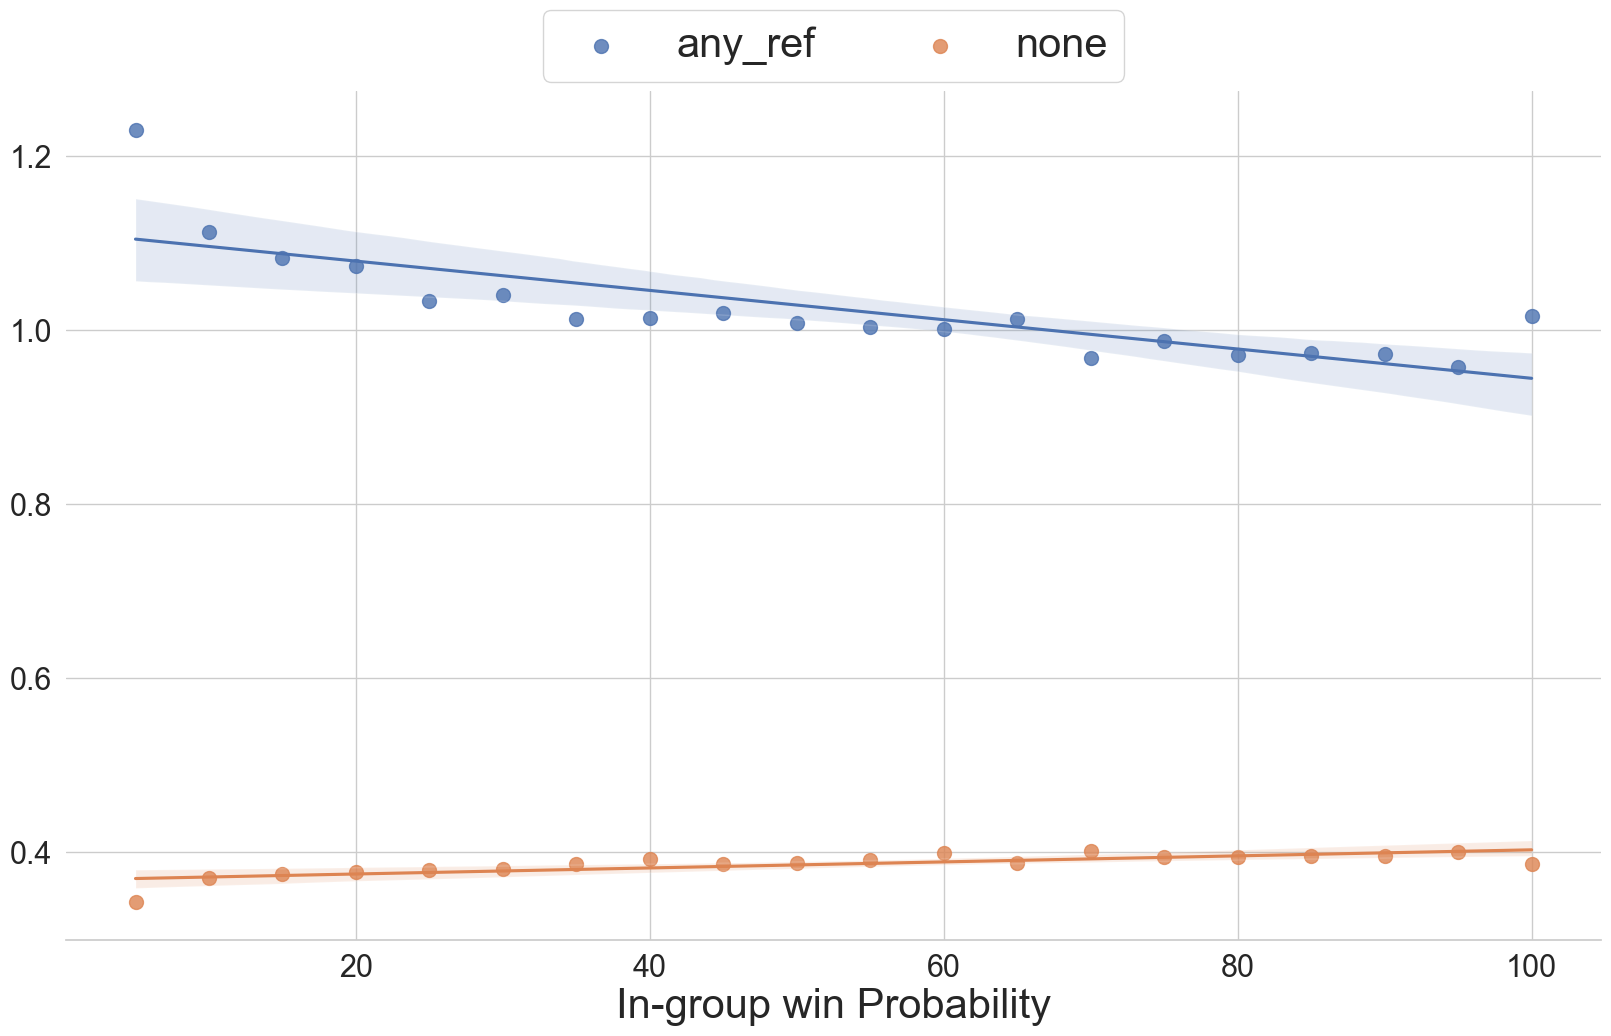
\includegraphics[width=0.85\linewidth]{figures/trends-1.png}
        \caption{Frequency of any-group and null references over all 5\% WP windows from 0 to 100}
        \label{fig:trends-1}
    \end{figure}
\end{frame}

\begin{frame}[c]\frametitle{All goes down}
    \begin{figure}[t]
        \centering
        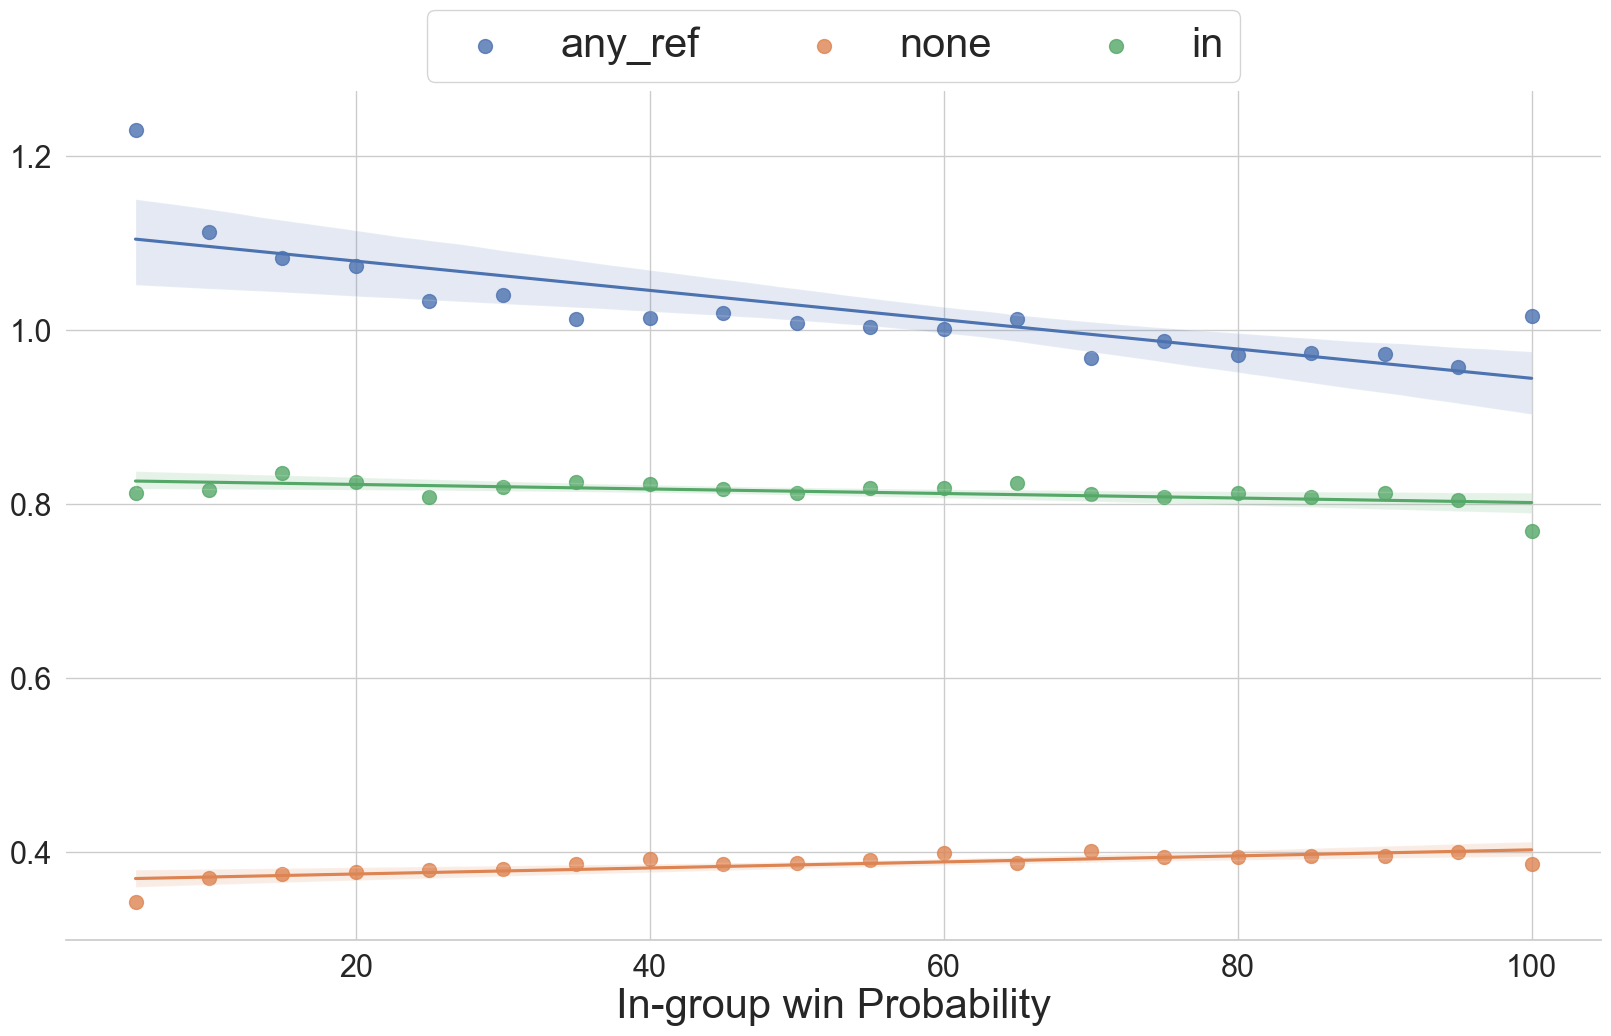
\includegraphics[width=0.85\linewidth]{figures/trends-2.png}
        \caption{Frequency of any-group, null and in-group (normalized within any-group) references over all 5\% WP windows from 0 to 100}
        \label{fig:trends-2}
    \end{figure}
\end{frame}

\begin{frame}[c]\frametitle{Reduction in reference frequency}
    The better the state of affairs in the real world for the \emph{in-group}, the more likely commenters are to \textbf{abstract away} from specifically referring to the in-group (or any group). \pause
    
    \ex.\label{ex:high-wp} \a. HOLY SHIT 
         \b. DO NOT TAKE YOUR FOOT OFF THE GAS
         \b. WHAT A THROW

\end{frame}

\begin{frame}[c]\frametitle{We few, we happy few, we...}
    \pause
    \begin{figure}[t]
         \centering
         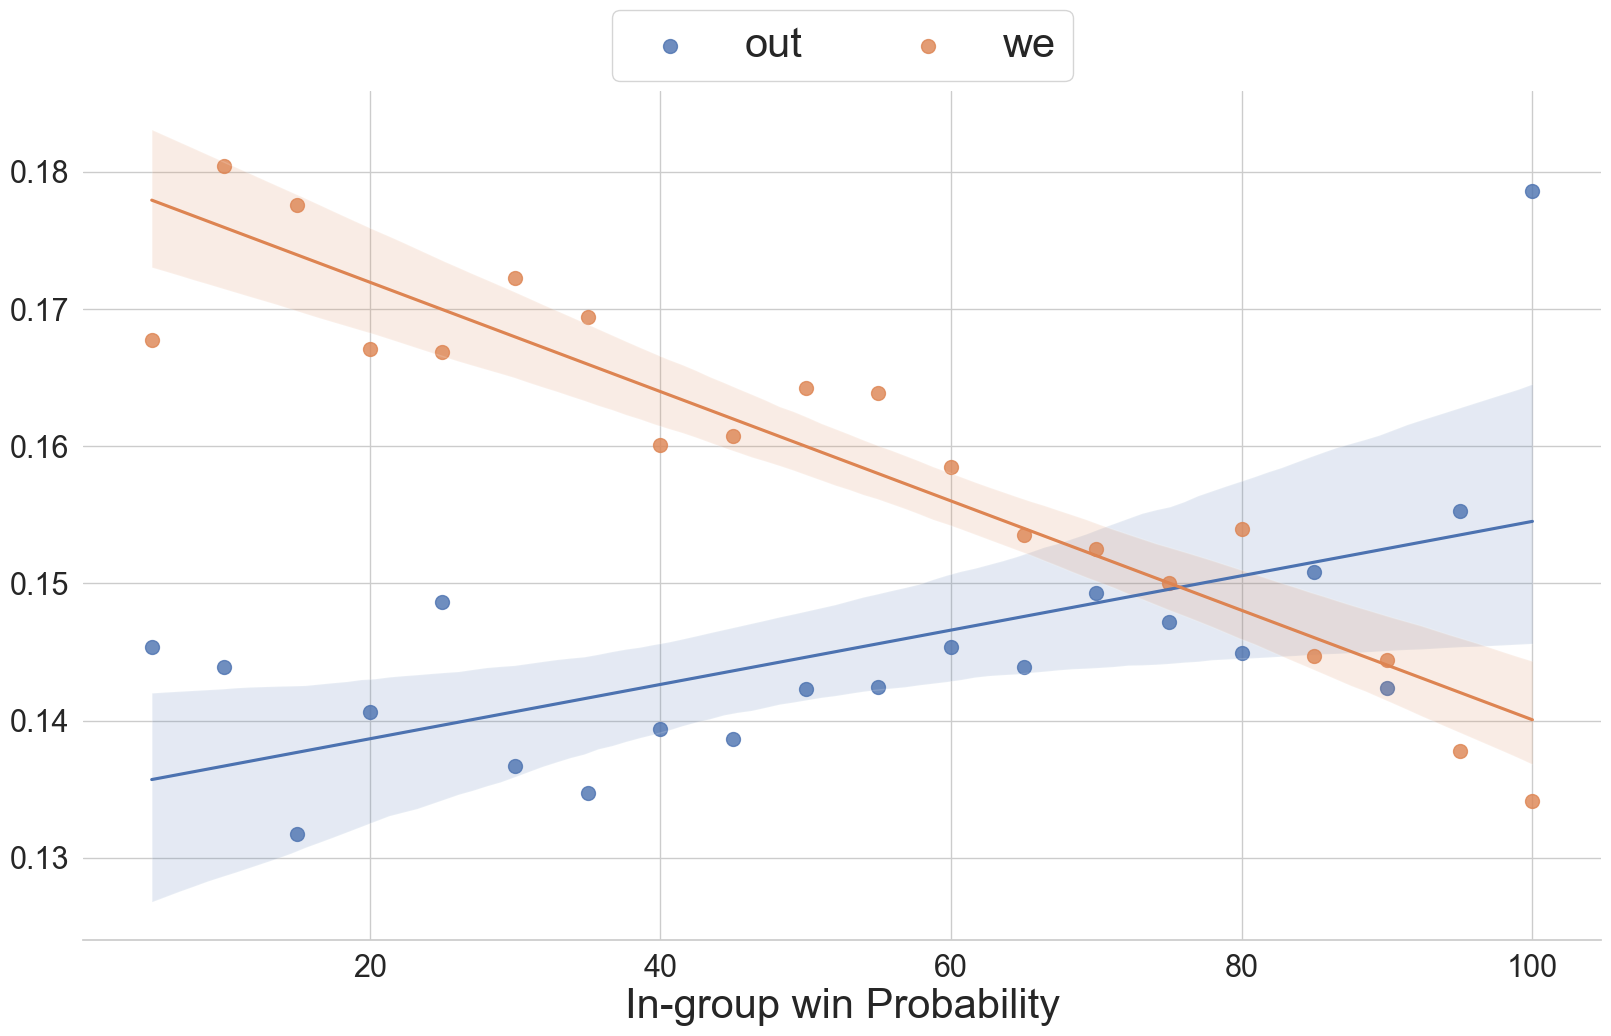
\includegraphics[width=0.85\linewidth]{figures/trends-3.png}
         \caption{Frequency of references to the in-group with first person plural forms, and the out-group, over all 5\% WP windows from 0 to 100.}
         \label{fig:trends-3}
     \end{figure}    
\end{frame}

\begin{frame}[c]\frametitle{We few, we happy few, we...}
    
    Fans band together to talk about the in-group with \textbf{third person plural referents} the less likely they are to win:

    \ex. \a. \alert{We} need a reliable safety ….. like , BAD .
         \b. \alert{Our defense} is not why \alert{we} lost the game . 

\end{frame}

\begin{frame}[c]\frametitle{Kick the out-group when they're down}

    Fans prefer to talk (shit) about the out-group, and refer less to the in-group, when the in-group is doing well:
    
    \ex. \a.  Keep going , hang 50 on \alert{these fuckers}.
         \b. ``Karma will get the Cowboys for trying to run up the score'' Actual comment in \alert{the Falcons} sub , tells you all you need to know about \alert{the pussies} over there.

\end{frame}

\begin{frame}[c]\frametitle{We're good, they suck}
    \pause
    \begin{figure}[t]
        \centering
        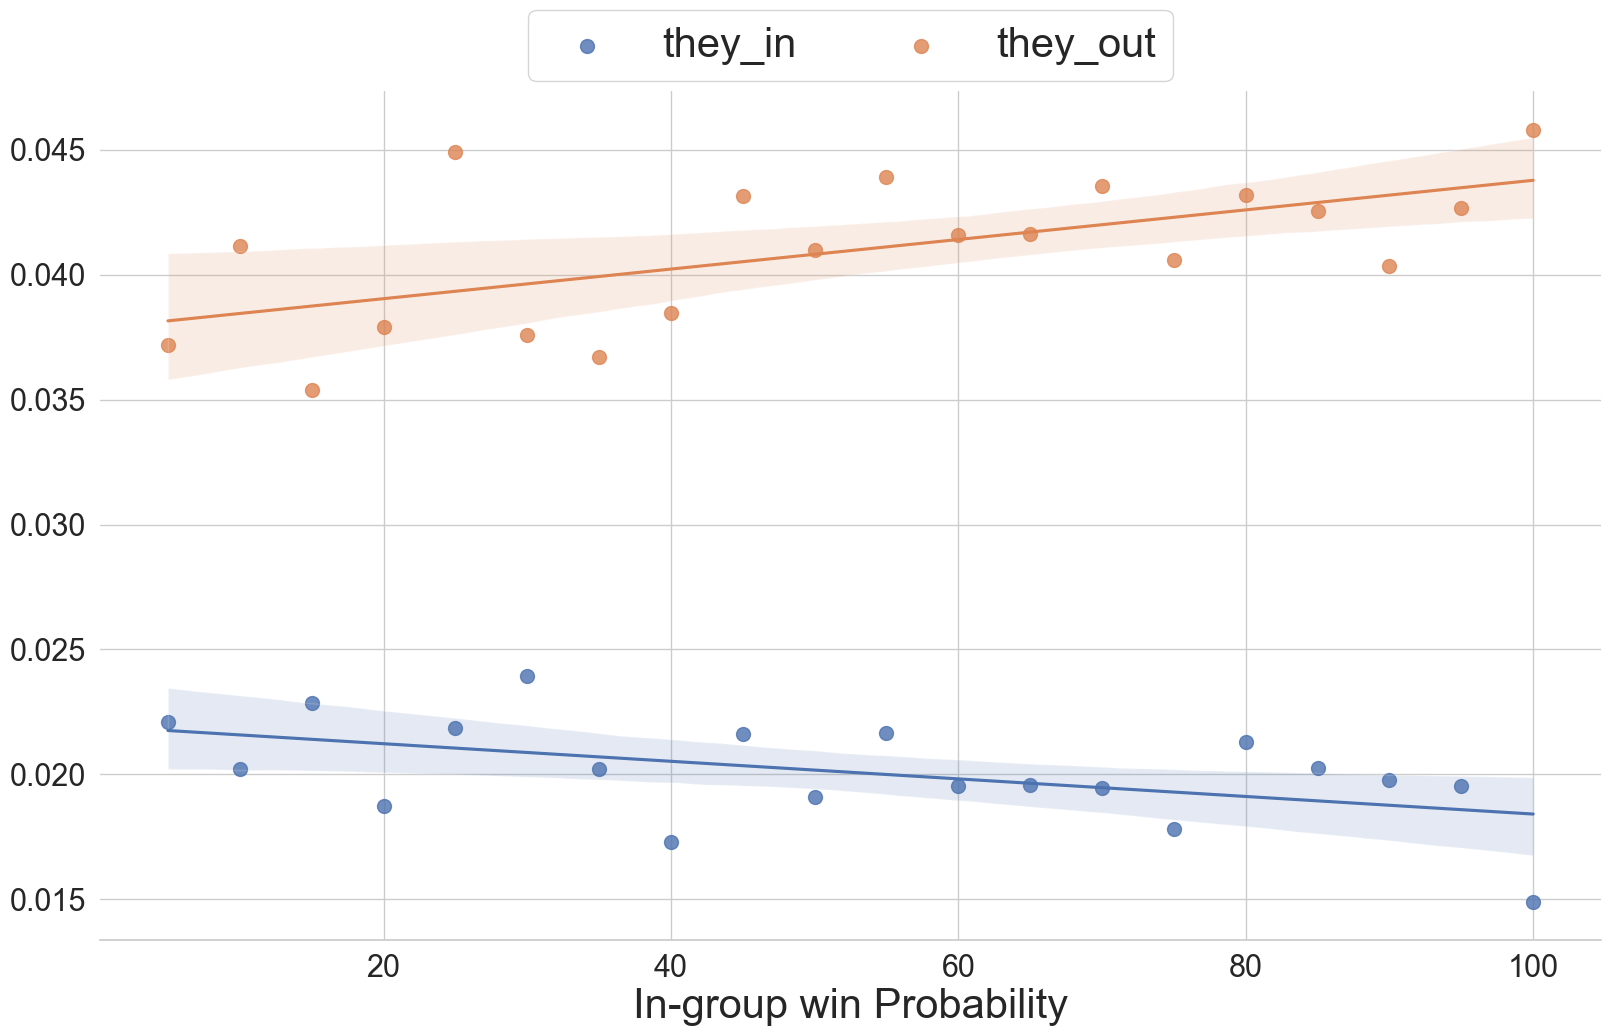
\includegraphics[width=0.85\linewidth]{figures/trends-4.png}
        \caption{Frequency of references to the in-group or out-group with \textbf{third person plural} over all 5\% WP windows from 0 to 100.}
        \label{fig:trends-4}
    \end{figure}
\end{frame}

